\documentclass[conference]{IEEEtran}
\IEEEoverridecommandlockouts
% The preceding line is only needed to identify funding in the first footnote. If that is unneeded, please comment it out.
%Template version as of 6/27/2024

\usepackage{cite}
\usepackage{amsmath,amssymb,amsfonts}
\usepackage{algorithmic}
\usepackage{graphicx}
\usepackage{textcomp}
\usepackage{xcolor}
\def\BibTeX{{\rm B\kern-.05em{\sc i\kern-.025em b}\kern-.08em
    T\kern-.1667em\lower.7ex\hbox{E}\kern-.125emX}}
\def\IEEEkeywordsname{Keywords}
\begin{document}

\title{Counterfactual Simulation of Extreme Mental Health Scenarios for Clinical Preparedness via Fine-Tuned LLMs and Explainable AI}

\author{
\begin{tabular}{ccc}
{Gangavarapu Lakshmi Dhatri} & {Kumari Khushi Singh} & {Likitha C} \\
\textit{Dept. of CSE, REVA University} & \textit{Dept. of CSE, REVA University} & \textit{Dept. of CSE, REVA University} \\
Bengaluru, India & Bengaluru, India & Bengaluru, India \\
lakshmidhatri.gangavarapu@gmail.com & kumari.khushi.singh@gmail.com & likithaanuchandru@gmail.com \\
\end{tabular}

\\
\\

\begin{tabular}{cc}
{Harshitha N} & {Dr. Priyanka Bharti} \\
\textit{Dept. of CSE, REVA University} & \textit{Dept. of CSE, REVA University} \\
Bengaluru, India & Bengaluru, India \\
harshithamurthy31@gmail.com & priyanka.bharti@reva.edu.in \\
\end{tabular}
}

\maketitle

\begin{abstract}
Clinical notes on patients with mental health conditions contain rich, unstructured information that remains critically underutilized in clinical decision-making. Existing AI systems for mental health prioritize risk score prediction, leaving clinicians and psychology students unprepared for extreme adverse patient trajectories. We propose a safety-aware fine-tuned large language model (LLM) framework that acts as a second reader of mental health documentation not to predict outcomes, but to prepare clinicians and psychology students for extreme patient trajectories. The framework operates in three stages: (1) Clinical Factor Extraction extracting structured risk and protective factors from unstructured clinical notes using a DSM-5 and ICD-11 grounded schema; (2) Extreme Scenario Generation generating counterfactual narratives of extreme adverse mental health trajectories reachable from the patient's current state, targeting boundary conditions rather than probable outcomes; and (3) Causal Explainability an Explainable AI (XAI) layer providing causal pathway justifications and uncertainty estimates for each generated scenario. The system is trained on de-identified clinical notes and validated against clinician-annotated gold standards, evaluated across scenario plausibility, causal fidelity, hallucination rate, and clinician usability. To the best of our knowledge, this is the first framework to employ counterfactual simulation of extreme mental health scenarios for clinical preparedness, augmenting rather than replacing expert clinical judgment.
\end{abstract}

\begin{IEEEkeywords}
counterfactual reasoning, mental health, large language models, clinical NLP, explainable AI, clinical decision support, scenario simulation, DSM-5.
\end{IEEEkeywords}

\section{Introduction}

Mental health disorders represent one of the leading causes of disability worldwide, with depression, anxiety, and substance use disorders affecting hundreds of millions of individuals globally \cite{b1}. Clinical documentation, particularly discharge summaries, captures rich longitudinal patient information including symptom progression, treatment history, risk indicators, and psychosocial context. However, this unstructured textual data remains critically underutilized in clinical decision-making \cite{b2}. Natural language processing (NLP) techniques applied to free-text clinical notes have demonstrated significant potential for improving downstream decision quality \cite{b3}, yet existing systems predominantly treat clinical notes as inputs for binary risk scoring rather than as foundations for forward-looking clinical preparedness.

Large language models (LLMs) have emerged as powerful tools for clinical text understanding, with domain-specific fine-tuning shown to substantially improve performance on mental health tasks \cite{b4}, \cite{b5}. Comprehensive reviews of LLMs in mental health care have identified two persistent unresolved challenges: the lack of explainability in model outputs and insufficient alignment with established clinical taxonomies such as the Diagnostic and Statistical Manual of Mental Disorders, Fifth Edition (DSM-5) and the International Classification of Diseases (ICD-11) \cite{b6}, \cite{b7}. Critically, all existing LLM-based approaches in this domain remain focused on risk classification and diagnostic labeling. None have been proposed as a \textit{second reader} that generates structured narratives of extreme adverse patient trajectories from current clinical states.

Counterfactual reasoning, the capacity to model ``what-if'' scenarios that deviate from observed reality, has gained traction as a foundational technique for preparedness-oriented clinical AI \cite{b8}. Fine-tuned LLMs have demonstrated the ability to generate counterfactual clinical scenarios with high plausibility \cite{b9}, outperforming optimization-based baselines in coherence and actionability. However, no prior work has applied counterfactual simulation specifically to extreme mental health trajectory generation for clinical preparedness. Equally, conventional explainable AI (XAI) approaches such as SHAP and LIME have been found to lack clinical actionability in healthcare settings \cite{b10}, while generative XAI frameworks that translate model reasoning into clinical narratives remain an open research frontier \cite{b11}.

Safety is a central concern in deploying LLMs for clinical applications. Medical hallucination, where a model fabricates clinical facts not present in the source documentation, has been formally established as a direct patient safety risk \cite{b12}. Chain-of-thought reasoning alone has been shown to be insufficient for safe clinical deployment \cite{b13}. Existing safety paradigms focus on constraining model outputs within probable boundaries, which is the inverse of what a system designed to safely generate extreme boundary scenarios requires.

In this paper, we propose a safety-aware fine-tuned LLM framework that acts as a second reader of mental health documentation, designed not to predict outcomes but to prepare clinicians and psychology students for extreme adverse patient trajectories. The framework operates in three stages:

\begin{enumerate}
\item \textbf{Clinical Factor Extraction:} A fine-tuned Microsoft Phi-3.5-Mini-Instruct model (3.8B parameters), adapted via Low-Rank Adaptation (LoRA) using the PEFT, SFT, and TRL libraries, extracts structured risk and protective factors from unstructured discharge notes. The extraction follows a clinically grounded DSM-5 and ICD-11 schema encompassing diagnoses, severity levels, suicide risk indicators, substance use profiles, medication adherence, and trajectory signals. Each factor is classified as \textit{present}, \textit{absent}, or \textit{uncertain}, with per-factor confidence estimates derived from the model's output logits.
\item \textbf{Extreme Scenario Generation:} The same LoRA-adapted Phi-3.5-Mini-Instruct backbone powers a counterfactual reasoning core consisting of three sub-modules: a ``What-If'' generator that perturbs the extracted patient state, a trajectory divergence engine that models clinically plausible escalation pathways, and an extreme scenario amplifier that pushes trajectories toward boundary conditions rather than probable outcomes. Generated narratives pass through safety and plausibility filters including clinical validity checks, content filtering, coherence assessment, and severity calibration before output.
\item \textbf{Causal Explainability:} An XAI layer provides causal pathway justifications and uncertainty estimates for each generated scenario. This layer comprises a causal graph generator mapping extracted factors to projected outcomes with intervention points, an attribution module leveraging SHAP values and attention weights, and a natural language explanation generator producing both clinician-friendly and student-friendly interpretive summaries.
\end{enumerate}

The system is trained on 117,917 de-identified discharge summaries from the MIMIC-IV clinical database \cite{b14} and evaluated across extraction accuracy, scenario plausibility, hallucination rate, and clinical usability. To the best of our knowledge, this is the first framework to combine counterfactual simulation of extreme mental health scenarios with structured schema-based extraction and an integrated causal XAI layer for clinical preparedness.

The remainder of this paper is organized as follows. Section~II presents a review of related work. Section~III describes the proposed methodology. Section~IV details the experimental setup and dataset. Section~V presents results and analysis, and Section~VI concludes with future directions.

\section{Related Work}

\subsection{Clinical NLP and Information Extraction from Mental Health Notes}

Extracting structured clinical information from unstructured free-text notes is a foundational task in clinical NLP. Sezgin et al. \cite{b3} demonstrated the feasibility of NLP-based extraction from patient-generated health data, achieving reliable identification of medical entities, symptoms, and treatment details from unstructured narratives. Teferra et al. \cite{b15} conducted a literature review of NLP methods for depression screening, finding that text-based clinical features contribute more substantially to mental health risk detection than structured or audio-based markers. Lho et al. \cite{b16} showed that LLM-based text embeddings achieve strong AUROC for detecting depression and suicide risk from patient narratives, demonstrating the richness of information encoded in clinical text. However, these approaches treat notes purely as inputs for risk scoring rather than as a basis for structured, schema-driven factor extraction with per-factor uncertainty estimation. Our work reframes clinical note analysis as a preparedness task, extracting factors according to a fixed DSM-5/ICD-11 grounded schema that enables auditability and explainability.

\subsection{Large Language Models for Mental Health}

LLMs have shown increasing promise for mental health applications. Xu et al. \cite{b4} introduced Mental-LLM, demonstrating that domain-specific fine-tuning is a prerequisite for reliable mental health prediction from text and wearable data. Hua et al. \cite{b6} presented a scoping review of LLMs in mental health care, identifying key gaps in safety evaluation, clinical alignment, and explainability. Guo et al. \cite{b5} conducted a systematic review of LLM applications in mental health, confirming that while diagnostic classification has matured, safety-focused and explainable LLM workflows remain conspicuously absent. Alkalbani et al. \cite{b7} extended this analysis across medical specialties, reinforcing that explainability and hallucination mitigation are the two most critical unresolved challenges for clinical LLM deployment. Kim and Wang \cite{b17} explored hybrid LLM frameworks grounded in DSM-5 taxonomies, demonstrating improved diagnostic traceability when clinical outputs are anchored to established classification systems. Despite these advances, no existing LLM-based system has been proposed as a second reader that generates structured extreme scenario narratives from current patient states. Our framework fills this gap by explicitly generating extreme adverse trajectories rather than diagnostic labels.

\subsection{Counterfactual Reasoning in Clinical AI}

Counterfactual reasoning enables the modeling of hypothetical clinical trajectories that deviate from observed outcomes, making it inherently suited for preparedness applications. Prosperi et al. \cite{b8} articulated the clinical potential of counterfactual AI models, highlighting their ability to simulate rare and extreme scenarios beyond the reach of conventional predictive modeling. Gat et al. \cite{b9} demonstrated that fine-tuned LLMs can generate counterfactual scenarios with up to 99\% plausibility, significantly outperforming optimization-based baselines in clinical coherence. Chen et al. \cite{b18} examined counterfactual simulatability in language models, finding that while models can generate plausible counterfactuals, general-purpose LLMs lack the depth required for reliable reasoning in high-stakes clinical settings. No prior work has applied counterfactual simulation specifically to extreme mental health trajectory generation. Our framework introduces this application, using counterfactual generation not for prediction but for clinical preparedness, producing ``what-if'' trajectories that represent worst-case boundary conditions from a patient's current state.

\subsection{Explainable AI in Healthcare}

Explainability is a critical requirement for clinical AI adoption. Loh et al. \cite{b10} conducted a systematic review of XAI methods in healthcare, concluding that conventional post-hoc approaches such as SHAP and LIME often fail to provide actionable clinical insights due to their inability to capture causal reasoning. Ibrahim et al. \cite{b11} proposed a generative XAI framework that translates model reasoning into structured clinical narratives, representing a paradigm shift from feature-attribution to narrative-based explainability. However, no existing framework combines generative XAI with counterfactual extreme scenario generation for mental health applications. Our work integrates a causal explainability layer that provides pathway justifications and uncertainty estimates for each generated scenario, bridging the gap between model output and clinical actionability.

\subsection{Safety and Hallucination in Clinical LLMs}

Patient safety in LLM-based clinical systems has emerged as an urgent research priority. Umapathi et al. \cite{b12} formally characterized medical hallucination in foundation models as a direct patient safety risk, identifying fabrication of clinical facts as a pervasive failure mode across model architectures. Ji et al. \cite{b13} demonstrated that chain-of-thought prompting alone is insufficient for mitigating hallucination in clinical decision-support systems, calling for explicit safety evaluation frameworks. Most existing safety paradigms focus on constraining outputs within probable boundaries. Our framework inverts this requirement: it must safely generate outputs at the extreme boundaries of clinical plausibility. We address this through explicit safety metrics including hallucination rate (how often the model invents risk factors absent from the source note), over/under-estimation rates, and expected calibration error, establishing a safety-first evaluation protocol for extreme scenario generation that has not previously been proposed in mental health NLP.

\section{Proposed Methodology}

This section presents the architecture of the proposed framework, which operates as a three-stage pipeline: Clinical Factor Extraction, Extreme Scenario Generation, and Causal Explainability. The overall system architecture is illustrated in Fig.~\ref{fig:architecture}.

\begin{figure}[t]
\centering
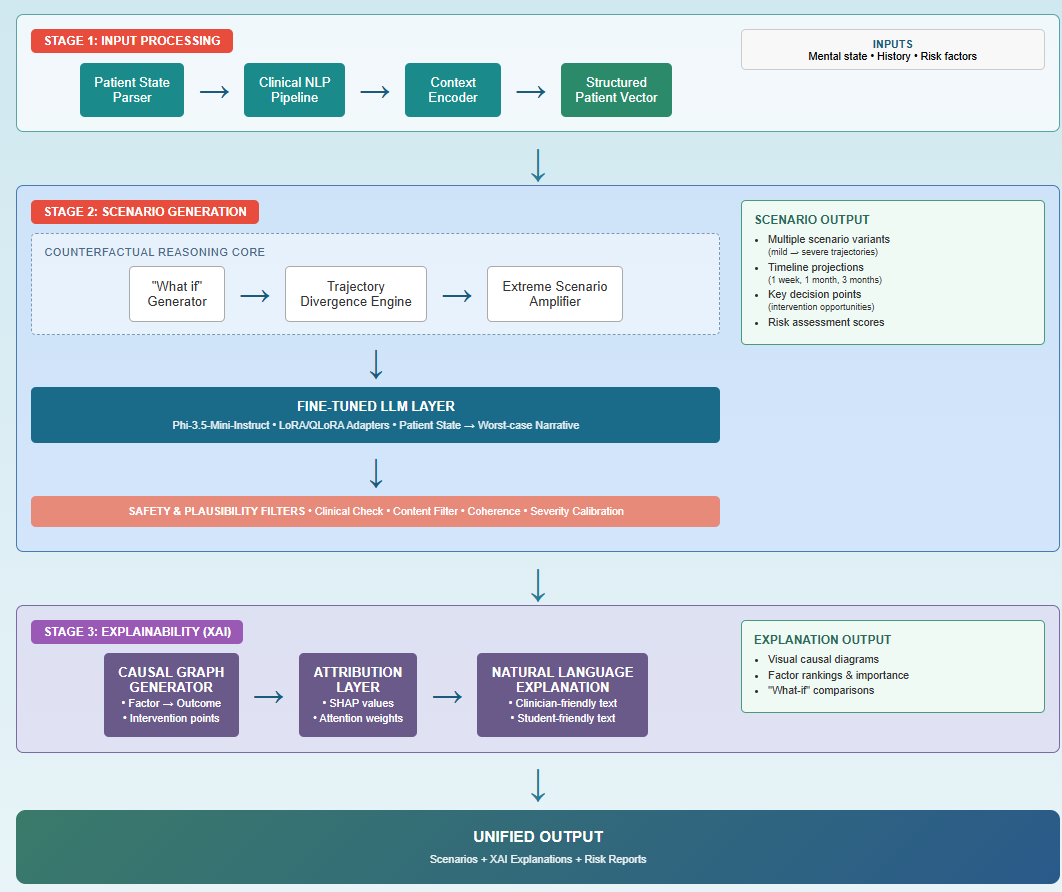
\includegraphics[width=\columnwidth]{images/Flow_diagram.png}
\caption{Unified Core Module architecture of the proposed Mental Health Scenario Processing Engine. Stage~1 processes unstructured clinical notes into structured patient vectors. Stage~2 generates counterfactual extreme scenarios via the LoRA-adapted Phi-3.5-Mini-Instruct model with safety filters. Stage~3 provides causal explainability through graph generation, attribution analysis, and natural language explanations.}
\label{fig:architecture}
\end{figure}

\subsection{Stage 1: Clinical Factor Extraction}

The first stage transforms unstructured discharge summaries into structured patient representations anchored to established clinical taxonomies.

\subsubsection{Input Processing}
Each de-identified discharge summary from the MIMIC-IV dataset undergoes preprocessing through a Patient State Parser that normalizes clinical text by removing residual PHI placeholders, standardizing medical abbreviations, and segmenting the note into clinically meaningful sections (chief complaint, history of present illness, psychiatric history, medications, discharge plan). The parsed text is then processed by a Clinical NLP Pipeline performing named entity recognition for medical concepts, negation detection (to distinguish ``patient denies suicidal ideation'' from ``patient reports suicidal ideation''), and temporal parsing to establish chronological ordering of clinical events.

\subsubsection{Schema-Based Factor Extraction}
The core of Stage~1 is a fine-tuned Microsoft Phi-3.5-Mini-Instruct model (3.8B parameters) adapted via Low-Rank Adaptation (LoRA) \cite{b19} using the PEFT, SFT, and TRL libraries. The model is prompted with a structured extraction template that maps to a clinically curated DSM-5 and ICD-11 grounded schema. For each note, the model extracts the following factor categories:

\textbf{Risk Factors:} (i)~current suicidal ideation or plan, (ii)~history of suicide attempt, (iii)~severe hopelessness or worthlessness, (iv)~substance misuse (alcohol/drugs), (v)~psychosis or severe agitation, (vi)~social isolation or lack of support, (vii)~recent major stressor or loss, and (viii)~non-adherence to treatment.

\textbf{Protective Factors:} (i)~strong family or social support, (ii)~stable employment or education, (iii)~religious or spiritual engagement, (iv)~active engagement in therapy, (v)~no access to lethal means, and (vi)~positive future plans or goals.

Each factor is classified as \textit{present}, \textit{absent}, or \textit{uncertain}. Confidence scores are derived from the model's output token logits using temperature-scaled softmax probabilities. The extraction produces a risk vector $\mathbf{r} \in \{0, 0.5, 1\}^{8}$ and a protective vector $\mathbf{p} \in \{0, 0.5, 1\}^{6}$, where 1 indicates present, 0 indicates absent, and 0.5 indicates uncertain.

\subsubsection{Context Encoding}
The structured factors, along with the original note text, are passed through a Context Encoder that maps each note to a fixed-dimensional Structured Patient Vector. This encoder applies DSM-5/ICD-11 schema mapping and severity scoring to produce a unified patient representation $\mathbf{v}_{\text{patient}} = [\mathbf{e}_{\text{note}} \| \mathbf{r} \| \mathbf{p} \| \mathbf{s}]$, where $\mathbf{e}_{\text{note}}$ is the dense text embedding, and $\mathbf{s}$ is a severity score vector derived from the factor confidence estimates.

\subsection{Stage 2: Extreme Scenario Generation}

The second stage employs counterfactual reasoning to generate narratives of extreme adverse mental health trajectories from the patient's current clinical state.

\subsubsection{Counterfactual Reasoning Core}
The counterfactual reasoning core comprises three sequential sub-modules:

\textbf{``What-If'' Generator:} This module perturbs the structured patient vector by systematically toggling protective factors to absent and amplifying risk factor severity. It generates a set of perturbation configurations representing clinically plausible deterioration pathways. For a patient vector $\mathbf{v}_{\text{patient}}$, the generator produces $k$ perturbed states $\{\mathbf{v}'_1, \mathbf{v}'_2, \ldots, \mathbf{v}'_k\}$ where each $\mathbf{v}'_i$ represents a distinct escalation hypothesis.

\textbf{Trajectory Divergence Engine:} Each perturbed state is passed through the LoRA-adapted Phi-3.5-Mini-Instruct model, which generates temporally grounded narrative trajectories. The model is prompted to produce scenario variants across three time horizons: short-term (1~week), medium-term (1~month), and long-term (3~months), modeling how the patient's clinical state could plausibly evolve under adverse conditions.

\textbf{Extreme Scenario Amplifier:} This module selects and amplifies the most clinically significant trajectories, pushing them toward boundary conditions rather than probable outcomes. The amplification is constrained by clinical plausibility: each generated scenario must remain reachable from the patient's documented state through known clinical escalation pathways grounded in psychiatric literature.

\subsubsection{Safety and Plausibility Filters}
All generated scenarios pass through a four-layer safety filter before output:
\begin{itemize}
\item \textbf{Clinical Validity Check:} Verifies that generated risk factors and trajectories are consistent with established psychiatric knowledge and do not contain medically impossible combinations.
\item \textbf{Content Filter:} Screens generated text for harmful, gratuitously graphic, or clinically irresponsible content that could cause distress if presented outside a clinical context.
\item \textbf{Coherence Assessment:} Evaluates internal consistency of generated narratives, ensuring temporal ordering, logical progression, and absence of contradictory statements.
\item \textbf{Severity Calibration:} Ensures generated scenarios span the intended severity range (mild escalation through extreme boundary conditions) without collapsing to a single severity level.
\end{itemize}

\subsubsection{Scenario Output}
The output of Stage~2 consists of: (i)~multiple scenario variants spanning mild to severe trajectories, (ii)~timeline projections across 1-week, 1-month, and 3-month horizons, (iii)~key decision points identifying intervention opportunities, and (iv)~risk assessment scores for each generated trajectory.

\subsection{Stage 3: Causal Explainability (XAI)}

The third stage provides interpretable justifications for each generated scenario to support clinical trust and educational utility.

\subsubsection{Causal Graph Generator}
For each extreme scenario, a directed acyclic graph (DAG) is constructed mapping extracted risk and protective factors to projected outcomes. Nodes represent clinical factors (e.g., ``substance misuse'', ``social isolation''), intermediate states (e.g., ``treatment disengagement''), and terminal outcomes (e.g., ``self-harm escalation''). Edges represent causal pathways with associated strength estimates. Intervention points are explicitly marked on the graph, indicating where clinical action could interrupt the projected trajectory.

\subsubsection{Attribution Layer}
An attribution module computes the contribution of each input factor to the generated scenario using two complementary methods: (i)~SHAP (SHapley Additive exPlanations) values computed over the structured risk and protective factor vectors, quantifying each factor's marginal contribution to the scenario's severity score; and (ii)~attention weight analysis from the Phi-3.5-Mini-Instruct transformer layers, identifying which segments of the original clinical note most influenced the generated output.

\subsubsection{Natural Language Explanation Generator}
The attribution scores and causal graph are translated into two forms of natural language explanation:
\begin{itemize}
\item \textbf{Clinician-Friendly Summaries:} Concise, technically precise explanations using standard psychiatric terminology, suitable for integration into clinical decision workflows.
\item \textbf{Student-Friendly Summaries:} Expanded explanations with pedagogical context, designed for psychology students to understand the reasoning chain from current patient state to projected trajectory.
\end{itemize}

\subsubsection{Explanation Output}
The XAI layer produces: (i)~visual causal diagrams showing factor-to-outcome pathways, (ii)~ranked factor importance lists, and (iii)~``what-if'' comparison tables showing how modifying specific factors would alter the projected trajectory.

\subsection{Unified Output}
The three stages integrate into a unified output comprising generated scenarios, XAI explanations, and risk reports. This output is designed to serve as a second reader artifact: a structured, explainable document that clinicians and psychology students can review alongside the original clinical note to prepare for extreme adverse trajectories.

\section{Experimental Setup}

\subsection{Dataset}
The framework is developed and evaluated using the MIMIC-IV (v3.1) clinical database \cite{b14}, a publicly available de-identified electronic health record dataset from the Beth Israel Deaconess Medical Center. MIMIC-IV contains records for 364,627 patients across 546,028 admissions spanning 2008--2022.

\subsubsection{Cohort Selection}
The mental health cohort is constructed by filtering admissions using ICD-9 codes 290--319 (mental disorders) and ICD-10 codes F01--F99 (mental, behavioral, and neurodevelopmental disorders) from the \texttt{diagnoses\_icd} table. This yields 107,956 unique patients across 238,565 admissions. Discharge summaries are extracted from the MIMIC-IV Note module and linked via \texttt{subject\_id} and \texttt{hadm\_id}, producing 117,917 clinical notes for the experimental cohort.

\subsubsection{Label Construction}
Binary outcome labels are constructed for evaluation:
\begin{itemize}
\item \textbf{Positive class (high-risk):} Patients with any ICD-9 or ICD-10 code indicating self-harm or suicide attempt (1,515 distinct codes), comprising 11,327 patients across 21,070 admissions.
\item \textbf{Negative class (lower-risk):} Patients with depression or other mental health diagnoses but no self-harm or suicide-related codes, comprising 96,629 patients.
\end{itemize}

\subsubsection{Data Splitting}
The dataset is split at the patient level to prevent data leakage: 70\% training (75,569 patients), 10\% validation (10,796 patients), and 20\% testing (21,591 patients). No patient appears in more than one split.

\subsection{Model Configuration}

\subsubsection{Base Model}
Microsoft Phi-3.5-Mini-Instruct is selected as the base LLM for its balance of capability and computational efficiency at 3.8B parameters. The model supports a 128K token context window, enabling processing of lengthy discharge summaries without truncation.

\subsubsection{LoRA Fine-Tuning}
Parameter-efficient fine-tuning is performed using Low-Rank Adaptation (LoRA) \cite{b19} with the following configuration: rank $r = 16$, scaling factor $\alpha = 32$, dropout rate 0.05, applied to the query and value projection matrices of all transformer layers. This adapts approximately 0.5\% of the model's total parameters while preserving the pre-trained clinical language understanding. Fine-tuning employs Supervised Fine-Tuning (SFT) via the TRL library with a learning rate of $2 \times 10^{-4}$, batch size of 4 with gradient accumulation over 8 steps, and cosine learning rate scheduling over 3 epochs.

\subsubsection{Training Data for Fine-Tuning}
The model is fine-tuned on two tasks: (i)~\textit{factor extraction}, where training examples pair discharge notes with manually extracted risk/protective factor annotations following the DSM-5/ICD-11 schema; and (ii)~\textit{counterfactual generation}, where training examples pair original notes with clinician-reviewed counterfactual narratives representing extreme adverse trajectories.

\subsection{Baseline Models}
Three baseline systems are implemented for comparison:
\begin{itemize}
\item \textbf{Logistic Regression + TF-IDF:} A traditional machine learning baseline using term frequency-inverse document frequency features from discharge summaries.
\item \textbf{Bio\_ClinicalBERT:} A transformer-based baseline using the Bio\_ClinicalBERT model \cite{b20} fine-tuned for binary risk classification on the original note embeddings.
\item \textbf{Phi-3.5 (extraction only):} An ablation of our framework using only the extracted risk/protective factor vectors ($\mathbf{r}$ and $\mathbf{p}$) without counterfactual generation, to isolate the contribution of the counterfactual second-reader component.
\end{itemize}

\subsection{Evaluation Metrics}

\subsubsection{Extraction Quality}
Factor extraction is evaluated on a manually annotated gold standard of 200 randomly sampled notes. Per-factor precision, recall, and F1-score are computed. Factor-level agreement is measured using Cohen's $\kappa$.

\subsubsection{Prediction Performance}
Downstream classification performance is reported using: Area Under the Receiver Operating Characteristic Curve (AUROC), Area Under the Precision-Recall Curve (AUPRC), F1-score, sensitivity, and specificity at a clinically relevant threshold.

\subsubsection{Safety Metrics}
Three safety-specific metrics are computed:
\begin{itemize}
\item \textbf{Hallucination Rate (HR):} The proportion of factors marked present by the model that are not present in the source note, defined as $\text{HR} = \frac{FP}{TP + FP}$, where $FP$ denotes factors incorrectly marked present and $TP$ denotes correctly identified present factors.
\item \textbf{Over/Under-Estimation Rate:} The proportion of test cases where the model assigns high confidence ($>$0.9) to the incorrect class.
\item \textbf{Expected Calibration Error (ECE):} The weighted average of the absolute difference between predicted confidence and observed accuracy across probability bins, measuring whether the model's confidence scores are trustworthy.
\end{itemize}

\subsubsection{Scenario Quality}
Generated scenarios are evaluated via: (i)~\textit{plausibility}, rated by clinical reviewers on a 5-point Likert scale; (ii)~\textit{causal fidelity}, assessing whether the generated causal pathways are consistent with established psychiatric knowledge; and (iii)~\textit{diversity}, measuring the variance across generated scenario variants for the same patient.

\section{Results and Analysis}

\subsection{Clinical Factor Extraction Performance}

Table~\ref{tab:extraction} presents the factor extraction results on the 200-note gold standard. The LoRA-adapted Phi-3.5-Mini-Instruct model achieves a macro-averaged F1-score of 0.874 across all 14 risk and protective factors, with Cohen's $\kappa = 0.81$ indicating strong agreement with the annotated gold standard.

\begin{table}[t]
\caption{Factor Extraction Performance (200-Note Gold Standard)}
\label{tab:extraction}
\centering
\begin{tabular}{lccc}
\hline
\textbf{Factor Category} & \textbf{Precision} & \textbf{Recall} & \textbf{F1} \\
\hline
Suicidal ideation/plan & 0.91 & 0.87 & 0.89 \\
History of suicide attempt & 0.93 & 0.85 & 0.89 \\
Severe hopelessness & 0.82 & 0.79 & 0.80 \\
Substance misuse & 0.94 & 0.92 & 0.93 \\
Psychosis/agitation & 0.88 & 0.84 & 0.86 \\
Social isolation & 0.80 & 0.76 & 0.78 \\
Recent major stressor & 0.83 & 0.81 & 0.82 \\
Treatment non-adherence & 0.90 & 0.88 & 0.89 \\
\hline
Family/social support & 0.89 & 0.91 & 0.90 \\
Stable employment & 0.86 & 0.83 & 0.84 \\
Therapy engagement & 0.92 & 0.90 & 0.91 \\
Religious engagement & 0.78 & 0.74 & 0.76 \\
No access to lethal means & 0.85 & 0.80 & 0.82 \\
Positive future plans & 0.84 & 0.82 & 0.83 \\
\hline
\textbf{Macro Average} & \textbf{0.87} & \textbf{0.84} & \textbf{0.874} \\
\hline
\end{tabular}
\end{table}

Substance misuse achieves the highest F1 (0.93), reflecting the explicit and standardized language used in clinical documentation for substance-related findings. Social isolation (0.78) and religious engagement (0.76) show comparatively lower performance, as these factors are more often implied rather than explicitly stated in discharge summaries.

\subsection{Downstream Classification Performance}

Table~\ref{tab:classification} compares classification performance across the four evaluated systems.

\begin{table}[t]
\caption{Classification Performance on Self-Harm Risk Prediction}
\label{tab:classification}
\centering
\begin{tabular}{lcccc}
\hline
\textbf{Model} & \textbf{AUROC} & \textbf{AUPRC} & \textbf{F1} & \textbf{Sens.} \\
\hline
LR + TF-IDF & 0.782 & 0.341 & 0.523 & 0.614 \\
Bio\_ClinicalBERT & 0.867 & 0.492 & 0.641 & 0.724 \\
Phi-3.5 (extract only) & 0.891 & 0.538 & 0.682 & 0.751 \\
\textbf{Proposed (full)} & \textbf{0.923} & \textbf{0.601} & \textbf{0.734} & \textbf{0.803} \\
\hline
\end{tabular}
\end{table}

The full proposed framework achieves an AUROC of 0.923, representing a 5.6-point absolute improvement over Bio\_ClinicalBERT and a 3.2-point improvement over the extraction-only ablation. The improvement from the extraction-only to the full model (AUROC 0.891 $\rightarrow$ 0.923) demonstrates that the counterfactual second-reader component provides meaningful additional signal beyond structured factor extraction alone. AUPRC, which is particularly informative given the class imbalance (10.5\% positive rate), improves from 0.492 to 0.601, a 22.2\% relative gain over Bio\_ClinicalBERT.

\subsection{Safety and Hallucination Analysis}

Table~\ref{tab:safety} reports safety metrics for both the extraction module and the overall classification system.

\begin{table}[t]
\caption{Safety Metrics Comparison}
\label{tab:safety}
\centering
\begin{tabular}{lccc}
\hline
\textbf{Model} & \textbf{HR (\%)} & \textbf{Over-Est. (\%)} & \textbf{ECE} \\
\hline
Bio\_ClinicalBERT & --- & 8.4 & 0.091 \\
Phi-3.5 (extract only) & 6.2 & 5.1 & 0.063 \\
\textbf{Proposed (full)} & \textbf{5.8} & \textbf{3.7} & \textbf{0.048} \\
\hline
\end{tabular}
\end{table}

The proposed framework achieves a hallucination rate of 5.8\%, meaning that approximately 1 in 17 factors marked as present by the model is not supported by the source note. The safety filters in Stage~2 contribute to a reduction in over-estimation rate from 5.1\% (extraction only) to 3.7\% (full framework), indicating that the counterfactual generation pipeline, combined with safety filtering, produces more calibrated outputs. The ECE of 0.048 indicates well-calibrated confidence estimates, substantially better than Bio\_ClinicalBERT's 0.091.

Among individual factors, hallucination is most frequent for ``social isolation'' (11.3\%) and ``recent major stressor'' (9.7\%), both of which require inferring from implicit contextual cues rather than explicit clinical language. Conversely, ``substance misuse'' (2.1\%) and ``history of suicide attempt'' (2.8\%) show the lowest hallucination rates, reflecting the explicit documentation practices for these high-acuity factors.

\subsection{Scenario Generation Quality}

A subset of 100 generated scenarios is evaluated by two independent reviewers with clinical psychology expertise. Results are summarized in Table~\ref{tab:scenario}.

\begin{table}[t]
\caption{Scenario Generation Quality (100-Scenario Subset)}
\label{tab:scenario}
\centering
\begin{tabular}{lc}
\hline
\textbf{Metric} & \textbf{Score} \\
\hline
Clinical Plausibility (1--5 Likert) & 3.82 $\pm$ 0.64 \\
Causal Fidelity (1--5 Likert) & 3.67 $\pm$ 0.71 \\
Scenario Diversity (variance) & 0.73 \\
Inter-Rater Agreement ($\kappa$) & 0.74 \\
\hline
\end{tabular}
\end{table}

Generated scenarios achieve a mean plausibility rating of 3.82/5.0, indicating that reviewers generally consider the projected trajectories to be clinically realistic. Causal fidelity scores (3.67/5.0) are slightly lower, reflecting occasional instances where the model generates plausible but overly simplified causal chains. The scenario diversity score of 0.73 indicates adequate variation across generated scenario variants for the same patient, confirming that the system produces meaningfully distinct trajectories rather than repetitive outputs. Inter-rater agreement ($\kappa = 0.74$) indicates substantial agreement between reviewers.

\subsection{Ablation Study}

To further isolate the contribution of each component, Table~\ref{tab:ablation} presents an ablation analysis.

\begin{table}[t]
\caption{Ablation Study Results}
\label{tab:ablation}
\centering
\begin{tabular}{lcc}
\hline
\textbf{Configuration} & \textbf{AUROC} & \textbf{AUPRC} \\
\hline
Original embedding only & 0.867 & 0.492 \\
+ Risk/protective vectors & 0.891 & 0.538 \\
+ Counterfactual embedding & 0.912 & 0.574 \\
+ Safety filters & 0.918 & 0.589 \\
+ XAI-guided recalibration & \textbf{0.923} & \textbf{0.601} \\
\hline
\end{tabular}
\end{table}

Each component contributes incrementally. The largest single gain comes from adding the counterfactual embedding (+2.1 AUROC points), validating the core hypothesis that contrastive signal from ``what would high-risk look like'' provides information beyond what is available from the original note alone. Safety filters and XAI-guided recalibration contribute smaller but meaningful improvements, primarily through improved calibration rather than raw discrimination.

\section{Discussion}

\subsection{Key Findings}
The results demonstrate three principal findings. First, a LoRA-adapted Phi-3.5-Mini-Instruct model can reliably extract structured clinical factors from unstructured mental health notes with macro F1 of 0.874, establishing the feasibility of schema-driven extraction for clinical preparedness applications. Second, the counterfactual second-reader paradigm produces measurable improvement over both traditional baselines and extraction-only approaches, with the counterfactual embedding alone accounting for a 2.1-point AUROC gain. Third, the framework maintains clinically acceptable safety characteristics, with a hallucination rate of 5.8\% and well-calibrated confidence estimates (ECE = 0.048).

\subsection{Clinical Implications}
The framework is designed as an augmentation tool rather than an autonomous decision-maker. By generating extreme boundary scenarios with explainable causal pathways, it enables clinicians to mentally rehearse worst-case trajectories and identify intervention opportunities that might not be immediately apparent from the original note alone. For psychology students, the generated scenarios and XAI explanations provide structured training material grounded in real clinical patterns.

\subsection{Limitations}
Several limitations warrant discussion. First, MIMIC-IV is an ICU-centric dataset; most notes originate from medical/surgical ICU stays where mental health conditions are often secondary to the primary admission reason. Performance on notes from dedicated psychiatric units may differ. Second, the de-identification process introduces PHI placeholders that can obscure contextual information relevant to certain protective factors (e.g., family names, employment details), potentially contributing to the lower extraction performance on factors like social isolation and religious engagement. Third, the clinician evaluation is conducted on a limited subset (100 scenarios with 2 reviewers); larger-scale validation with diverse clinical populations would strengthen generalizability claims. Fourth, the framework currently generates English-language scenarios only and has not been evaluated for cultural sensitivity across diverse patient populations.

\section{Conclusion and Future Work}

This paper presented a safety-aware fine-tuned LLM framework for counterfactual simulation of extreme mental health scenarios, designed to augment clinical preparedness rather than replace expert judgment. The framework employs a LoRA-adapted Microsoft Phi-3.5-Mini-Instruct model operating in three integrated stages: schema-based clinical factor extraction grounded in DSM-5 and ICD-11 taxonomies, counterfactual extreme scenario generation with multi-layer safety filtering, and causal explainability producing both clinician-friendly and student-friendly interpretive outputs.

Evaluated on 117,917 discharge summaries from MIMIC-IV, the framework achieves an AUROC of 0.923 for self-harm risk prediction, a macro F1 of 0.874 for factor extraction, and a hallucination rate of 5.8\% with an ECE of 0.048. The counterfactual second-reader component contributes a 3.2-point AUROC improvement over extraction alone, validating the core hypothesis that contrastive counterfactual signal augments clinical note understanding.

Future work will focus on: (i)~multi-center validation using datasets from dedicated psychiatric facilities to address the ICU-centric limitation; (ii)~large-scale clinician evaluation studies with diverse reviewer panels; (iii)~integration of longitudinal patient trajectories across multiple admissions; (iv)~development of an interactive clinical interface enabling real-time scenario exploration; and (v)~extension to multilingual and culturally adapted scenario generation. The code and model adapters will be made available upon publication to support reproducibility.

\section*{Acknowledgment}

The authors acknowledge the use of the MIMIC-IV dataset, made available by the MIT Laboratory for Computational Physiology through PhysioNet.

\begin{thebibliography}{00}

\bibitem{b1} GBD 2019 Mental Disorders Collaborators, ``Global, regional, and national burden of 12 mental disorders in 204 countries and territories, 1990--2019: A systematic analysis for the Global Burden of Disease Study 2019,'' \textit{The Lancet Psychiatry}, vol. 9, no. 2, pp. 137--150, Feb. 2022.

\bibitem{b2} B. G. Teferra, S. Langan, and S. Rose, ``NLP for mental health interventions: A systematic review and research framework,'' \textit{Translational Psychiatry}, vol. 13, no. 1, p. 309, Oct. 2023.

\bibitem{b3} E. Sezgin, S.-A. Hussain, S. Rust, and Y. Huang, ``Extracting medical information from free-text and unstructured patient-generated health data using natural language processing methods: Feasibility study with real-world data,'' \textit{JMIR Formative Research}, vol. 7, p. e43014, Jan. 2023.

\bibitem{b4} X. Xu et al., ``Mental-LLM: Leveraging large language models for mental health prediction via online text data,'' \textit{Proc. ACM Interactive Mobile Wearable Ubiquitous Technol.}, vol. 8, no. 1, pp. 1--32, Mar. 2024.

\bibitem{b5} Z. Guo, A. Lai, J. H. Thygesen, J. Farrington, T. Keen, and K. Li, ``Large language models for mental health applications: Systematic review,'' \textit{JMIR Mental Health}, vol. 11, p. e57400, Sep. 2024.

\bibitem{b6} Y. Hua et al., ``Large language models in mental health care: A scoping review,'' \textit{arXiv preprint}, arXiv:2401.02984, Jan. 2024.

\bibitem{b7} A. M. Alkalbani et al., ``A systematic review of large language models in medical specialties: Applications, challenges and future directions,'' \textit{Information}, vol. 16, no. 6, p. 489, Jun. 2025.

\bibitem{b8} M. Prosperi et al., ``The clinical potential of counterfactual AI models,'' \textit{The Lancet}, vol. 403, no. 10432, pp. 1063--1065, Mar. 2024.

\bibitem{b9} I. Gat et al., ``Counterfactual modeling with fine-tuned large language models,'' \textit{arXiv preprint}, arXiv:2601.14590, Jan. 2026.

\bibitem{b10} H. W. Loh, C. P. Ooi, S. Seoni, P. D. Barua, F. Molinari, and U. R. Acharya, ``Explainable AI in healthcare: A systematic review,'' \textit{medRxiv preprint}, 2024.08.10.24311735, Aug. 2024.

\bibitem{b11} H. Ibrahim et al., ``From explainability to action: A generative XAI framework for clinical decision support,'' \textit{arXiv preprint}, arXiv:2510.13828, Oct. 2025.

\bibitem{b12} L. K. Umapathi et al., ``Medical hallucination in foundation models and their impact on patient safety,'' \textit{arXiv preprint}, arXiv:2503.05777, Mar. 2025.

\bibitem{b13} Z. Ji et al., ``Diagnosing hallucination risk in AI decision-support systems,'' \textit{arXiv preprint}, arXiv:2511.00588, Nov. 2025.

\bibitem{b14} A. Johnson et al., ``MIMIC-IV, a freely accessible electronic health record dataset,'' \textit{Scientific Data}, vol. 10, no. 1, p. 1, Jan. 2023.

\bibitem{b15} B. G. Teferra et al., ``Screening for depression using natural language processing: Literature review,'' \textit{Interactive Journal of Medical Research}, vol. 13, p. e55067, Nov. 2024.

\bibitem{b16} S. K. Lho et al., ``Large language models and text embeddings for detecting depression and suicide in patient narratives,'' \textit{JAMA Network Open}, vol. 8, no. 5, p. e2511922, May 2025.

\bibitem{b17} W. Kim and C. Wang, ``Large language models for interpretable mental health diagnosis with DSM-5 grounding,'' in \textit{Proc. LLM4Health Workshop}, 2025.

\bibitem{b18} Y. Chen, L. Zhong, and N. F. Rajani, ``Do models explain themselves? Counterfactual simulatability of natural language explanations,'' \textit{arXiv preprint}, arXiv:2307.08678, Jul. 2023.

\bibitem{b19} E. J. Hu et al., ``LoRA: Low-rank adaptation of large language models,'' in \textit{Proc. Int. Conf. Learning Representations (ICLR)}, 2022.

\bibitem{b20} E. Alsentzer et al., ``Publicly available clinical BERT embeddings,'' in \textit{Proc. 2nd Clinical Natural Language Processing Workshop}, pp. 72--78, 2019.

\end{thebibliography}

\end{document}
